\documentclass[11pt,a4paper]{report}
\usepackage[textwidth=37em,vmargin=30mm]{geometry}
\usepackage{calc,xunicode,amsmath,amssymb,paralist,enumitem,tabu,booktabs,datetime2,xeCJK,xeCJKfntef,listings}
\usepackage{tocloft,fancyhdr,tcolorbox,xcolor,graphicx,eso-pic,xltxtra,xelatexemoji}

\newcommand{\envyear}[0]{2025}
\newcommand{\envdatestr}[0]{2025-03-04}
\newcommand{\envfinaldir}[0]{webdb/2025/20250304/final}

\usepackage[hidelinks]{hyperref}
\hypersetup{
    colorlinks=false,
    pdfpagemode=FullScreen,
    pdftitle={Web Digest - \envdatestr}
}

\setlength{\cftbeforechapskip}{10pt}
\renewcommand{\cftchapfont}{\rmfamily\bfseries\large\raggedright}
\setlength{\cftbeforesecskip}{2pt}
\renewcommand{\cftsecfont}{\sffamily\small\raggedright}

\setdefaultleftmargin{2em}{2em}{1em}{1em}{1em}{1em}

\usepackage{xeCJK,xeCJKfntef}
\xeCJKsetup{PunctStyle=plain,RubberPunctSkip=false,CJKglue=\strut\hskip 0pt plus 0.1em minus 0.05em,CJKecglue=\strut\hskip 0.22em plus 0.2em}
\XeTeXlinebreaklocale "zh"
\XeTeXlinebreakskip = 0pt


\setmainfont{Brygada 1918}
\setromanfont{Brygada 1918}
\setsansfont{IBM Plex Sans}
\setmonofont{JetBrains Mono NL}
\setCJKmainfont{Noto Serif CJK SC}
\setCJKromanfont{Noto Serif CJK SC}
\setCJKsansfont{Noto Sans CJK SC}
\setCJKmonofont{Noto Sans CJK SC}

\setlength{\parindent}{0pt}
\setlength{\parskip}{8pt}
\linespread{1.15}

\lstset{
	basicstyle=\ttfamily\footnotesize,
	numbersep=5pt,
	backgroundcolor=\color{black!5},
	showspaces=false,
	showstringspaces=false,
	showtabs=false,
	tabsize=2,
	captionpos=b,
	breaklines=true,
	breakatwhitespace=true,
	breakautoindent=true,
	linewidth=\textwidth
}






\newcommand{\coverpic}[2]{
    % argv: itemurl, authorname
    Cover photo by #2~~(\href{#1}{#1})
}
\newcommand{\makeheader}[0]{
    \begin{titlepage}
        % \newgeometry{hmargin=15mm,tmargin=21mm,bmargin=12mm}
        \begin{center}
            
            \rmfamily\scshape
            \fontspec{BaskervilleF}
            \fontspec{Old Standard}
            \fontsize{59pt}{70pt}\selectfont
            WEB\hfill DIGEST
            
            \vfill
            % \vskip 30pt
            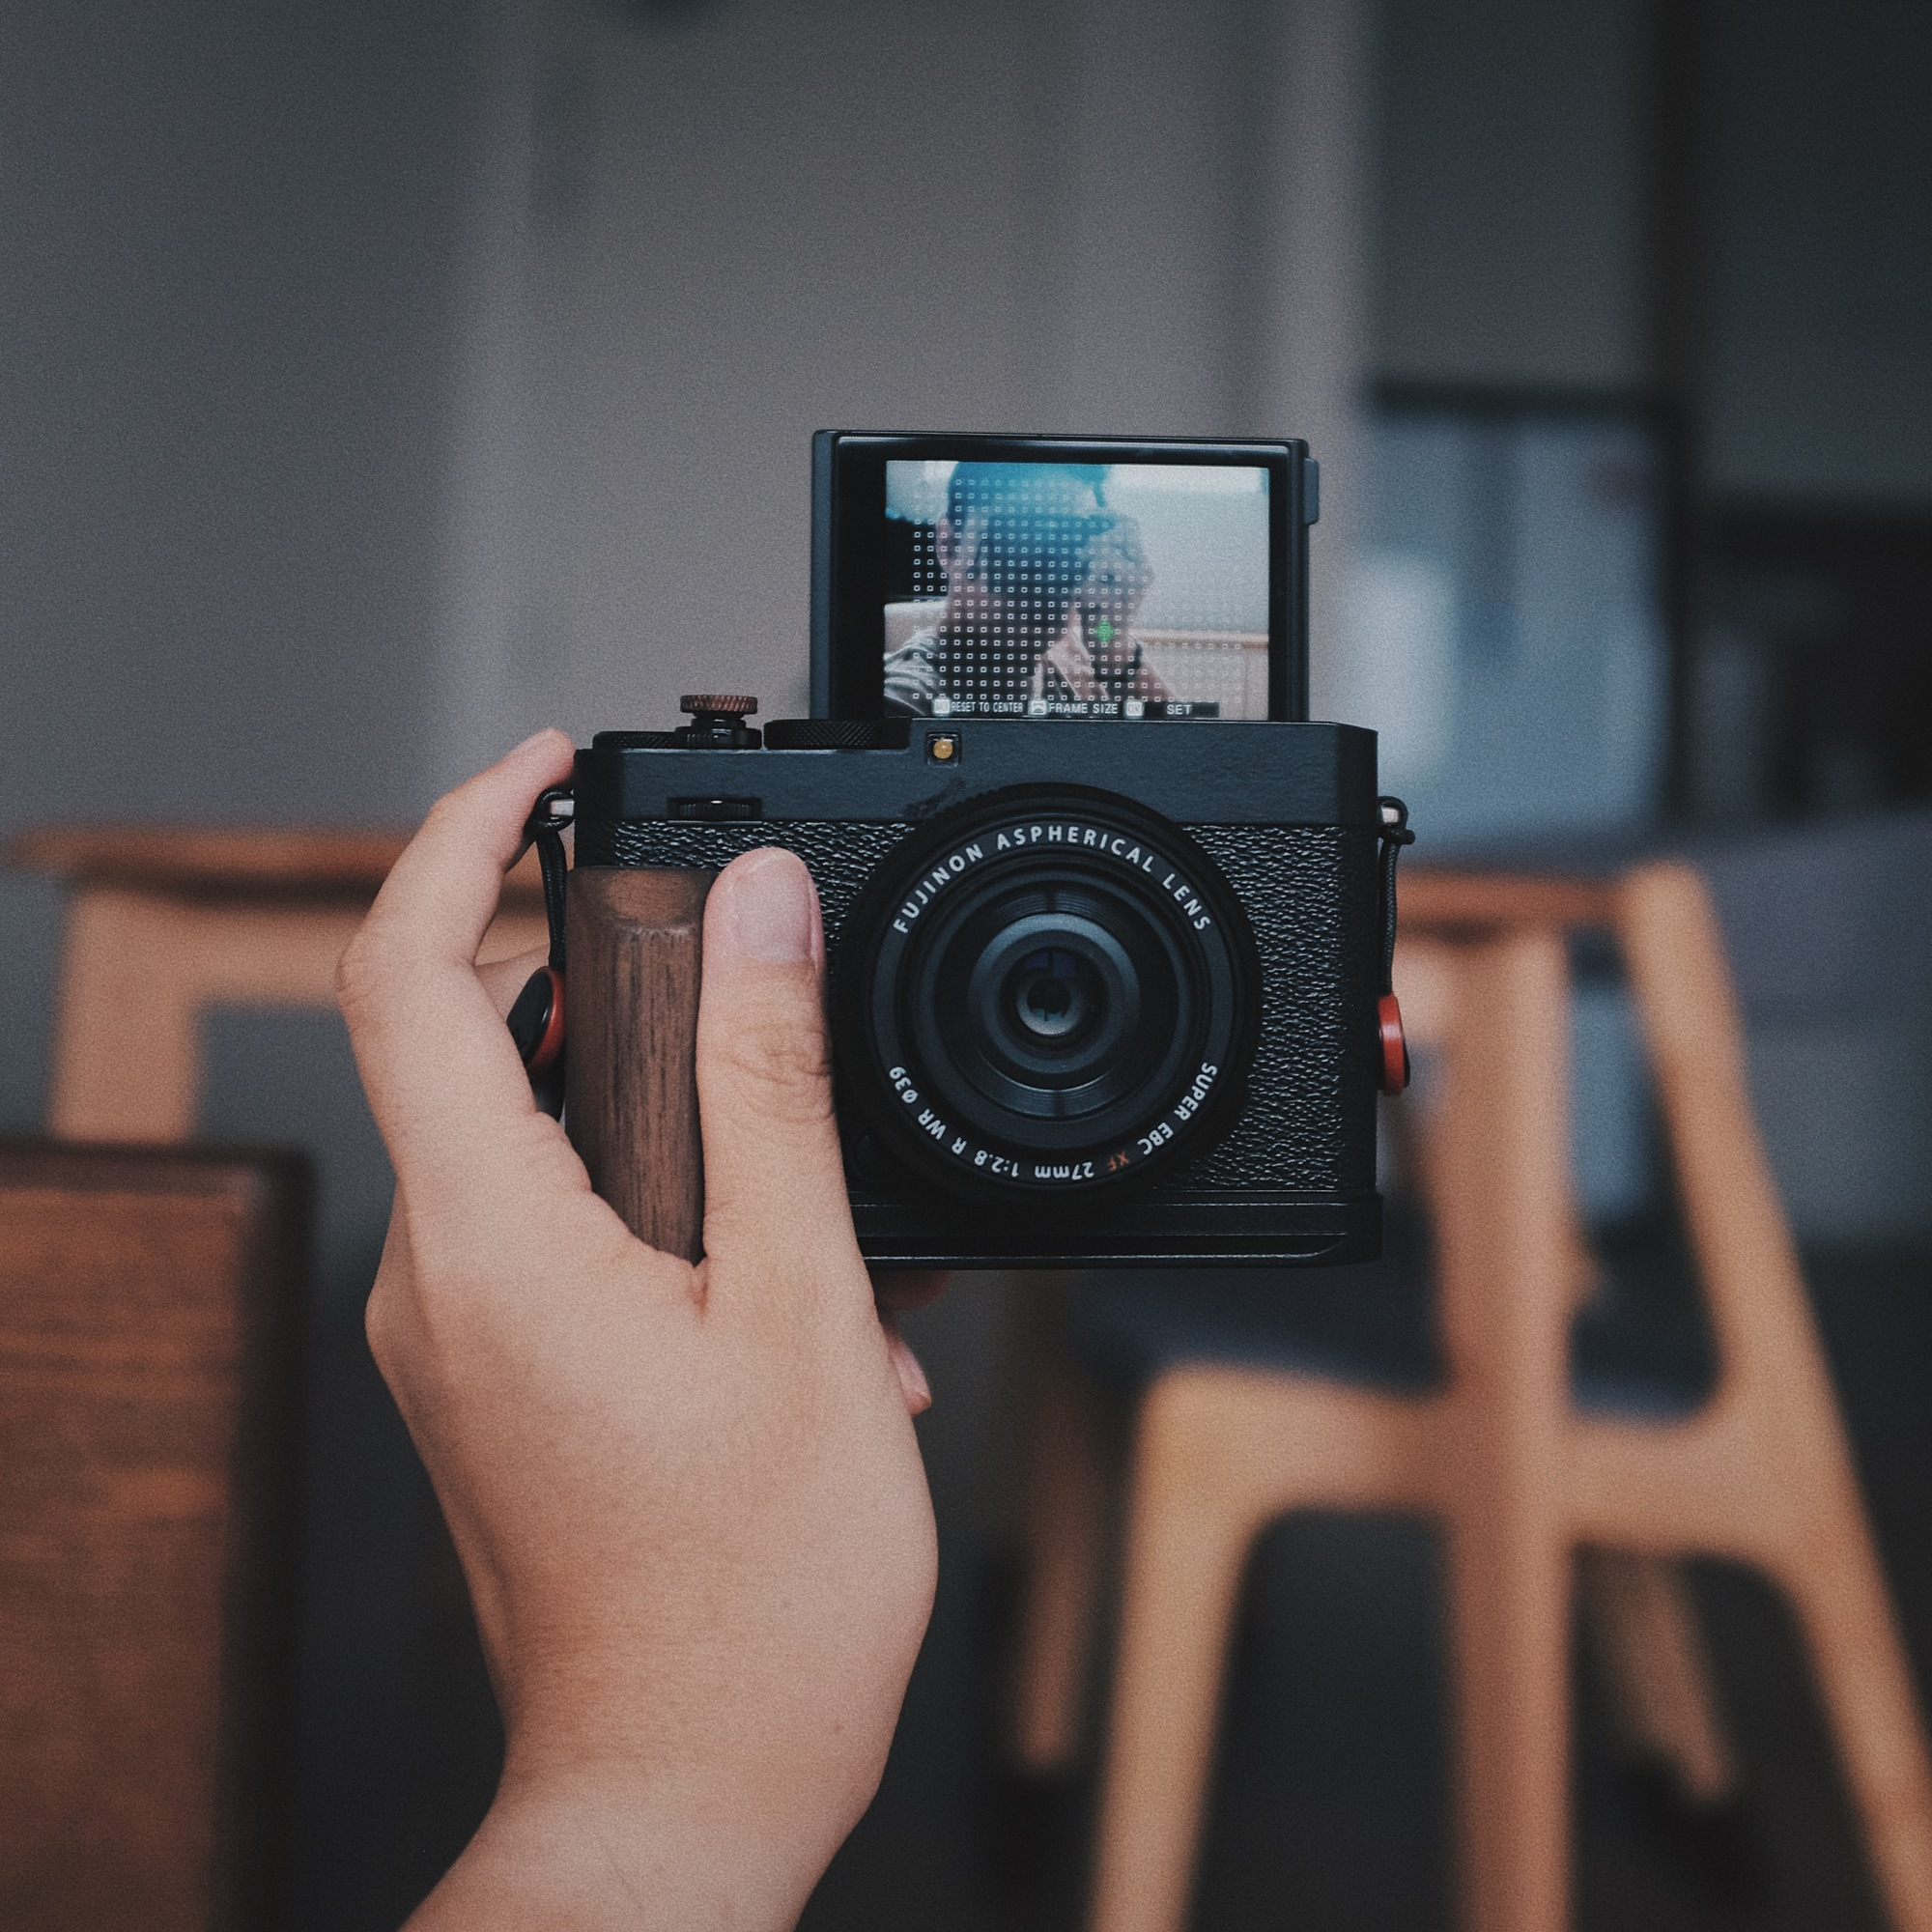
\includegraphics[width=\linewidth]{\envfinaldir/coverpic-prod.jpg}\par
            % \vskip 30pt
            \vfill

            \normalsize\rmfamily\scshape
            \copyright{} The Web Digest Project \hfill\large \envdatestr
        \end{center}
    \end{titlepage}
    % \restoregeometry
}
\newcommand{\simplehref}[1]{%
    \textcolor{blue!80!green}{\href{#1}{#1}}%
}
\renewcommand{\contentsname}{\center\Huge\sffamily\bfseries Contents\par\vskip 20pt}
\newcounter{ipartcounter}
\setcounter{ipartcounter}{0}
\newcommand{\ipart}[1]{
    % \vskip 20pt
    \clearpage
    \stepcounter{ipartcounter}
    \phantomsection
    \addcontentsline{toc}{chapter}{#1}
    % \begin{center}
    %     \Huge
    %     \sffamily\bfseries
    %     #1
    % \end{center}
    % \vskip 20pt plus 7pt
}
\newcounter{ichaptercounter}
\setcounter{ichaptercounter}{0}
\newcommand{\ichapter}[1]{
    % \vskip 20pt
    \clearpage
    \stepcounter{ichaptercounter}
    \phantomsection
    \addcontentsline{toc}{section}{\numberline{\arabic{ichaptercounter}}#1}
    \begin{center}
        \Huge
        \sffamily\bfseries
        #1
    \end{center}
    \vskip 20pt plus 7pt
}
\newcommand{\entrytitlefont}[1]{\subsection*{\raggedright\Large\sffamily\bfseries#1}}
\newcommand{\entryitemGeneric}[2]{
    % argv: title, url
    \parbox{\linewidth}{
        \entrytitlefont{#1}\par\vskip 5pt
        \footnotesize\ttfamily\mdseries
        \simplehref{#2}
    }\vskip 11pt plus 11pt minus 1pt
}
\newcommand{\entryitemGithub}[3]{
    % argv: title, url, desc
    \parbox{\linewidth}{
        \entrytitlefont{#1}\par\vskip 5pt
        \footnotesize\ttfamily\mdseries
        \simplehref{#2}\par\vskip 5pt
        \small\rmfamily\mdseries#3
    }\vskip 11pt plus 11pt minus 1pt
}
\newcommand{\entryitemAp}[3]{
    % argv: title, url, desc
    \parbox{\linewidth}{
        \entrytitlefont{#1}\par\vskip 5pt
        \footnotesize\ttfamily\mdseries
        \simplehref{#2}\par\vskip 5pt
        \small\rmfamily\mdseries#3
    }\vskip 11pt plus 11pt minus 1pt
}
\newcommand{\entryitemHackernews}[3]{
    % argv: title, hnurl, rawurl
    % \parbox{\linewidth}{
    %     \entrytitlefont{#1}\par\vskip 5pt
    %     \footnotesize\ttfamily\mdseries
    %     \simplehref{#3}\par
    %     \textcolor{black!50}{\href{#2}{#2}}
    % }\vskip 11pt plus 11pt minus 1pt
    \begin{minipage}{\linewidth}
            \entrytitlefont{#1}\par\vskip 5pt
            \footnotesize\ttfamily\mdseries
            \simplehref{#3}\par
            \textcolor{black!50}{\href{#2}{#2}}
    \end{minipage}\par\vskip 11pt plus 11pt minus 1pt
}







\begin{document}

\makeheader

\tableofcontents\clearpage




\ipart{Developers}
\ichapter{Hacker News}
\entryitemTwoLinks{Repairable Flatpack Toaster}{https://news.ycombinator.com/item?id=43246892}{https://www.kaseyhou.com/\#/repairable-flatpack-toaster/}

\entryitemTwoLinks{Atlanta Fed predicts -2.8\% GDP}{https://news.ycombinator.com/item?id=43246371}{https://www.atlantafed.org/cqer/research/gdpnow}

\entryitemTwoLinks{James Harrison, whose blood donations saved >2M babies, has died}{https://news.ycombinator.com/item?id=43245129}{https://www.npr.org/2025/03/03/nx-s1-5316163/james-harrison-blood-donor}

\entryitemTwoLinks{Hacking the Xbox 360 Hypervisor Part 2: The Bad Update Exploit}{https://news.ycombinator.com/item?id=43244739}{https://icode4.coffee/?p=1081}

\entryitemTwoLinks{Ex-SAP CTO walks away with €7.1M payout after scandal}{https://news.ycombinator.com/item?id=43244490}{https://www.theregister.com/2025/03/03/former\_sap\_cto\_payout/}

\entryitemTwoLinks{SQLite-on-the-Server Is Misunderstood: Better at Hyper-Scale Than Micro-Scale}{https://news.ycombinator.com/item?id=43244307}{https://rivet.gg/blog/2025-02-16-sqlite-on-the-server-is-misunderstood}

\entryitemTwoLinks{The power of interning: making a time series database smaller}{https://news.ycombinator.com/item?id=43243914}{https://gendignoux.com/blog/2025/03/03/rust-interning-2000x.html}

\entryitemTwoLinks{The Golden Age of Japanese Pencils, 1952-1967}{https://news.ycombinator.com/item?id=43243716}{https://notes.stlartsupply.com/the-golden-age-of-japanese-pencils-1952-1967/}

\entryitemTwoLinks{An Attempt to Catch Up with JIT Compilers}{https://news.ycombinator.com/item?id=43243109}{https://arxiv.org/abs/2502.20547}

\entryitemTwoLinks{Apple's Software Quality Crisis}{https://news.ycombinator.com/item?id=43243075}{https://www.eliseomartelli.it/blog/2025-03-02-apple-quality}

\entryitemTwoLinks{Ask HN: Who is hiring? (March 2025)}{https://news.ycombinator.com/item?id=43243024}{https://news.ycombinator.com/item?id=43243024}

\entryitemTwoLinks{Ask HN: Who wants to be hired? (March 2025)}{https://news.ycombinator.com/item?id=43243022}{https://news.ycombinator.com/item?id=43243022}

\entryitemTwoLinks{Show HN: Knowledge graph of restaurants and chefs, built using LLMs}{https://news.ycombinator.com/item?id=43242818}{https://theophilecantelob.re/blog/2025/foudinge/}

\entryitemTwoLinks{Youth and what happens when it's gone}{https://news.ycombinator.com/item?id=43242815}{https://tolstoyan.substack.com/p/youth}

\entryitemTwoLinks{The Internals of PostgreSQL}{https://news.ycombinator.com/item?id=43241404}{http://www.interdb.jp/pg/index.html}

\entryitemTwoLinks{Amazon's delivery drones are grounded in College Station, Texas}{https://news.ycombinator.com/item?id=43241212}{https://www.wired.com/story/texas-amazon-drones-stop-flying/}

\entryitemTwoLinks{About Google Chrome's "This extension may soon no longer be supported" (2024)}{https://news.ycombinator.com/item?id=43239774}{https://github.com/gorhill/uBlock/wiki/About-Google-Chrome\%27s-\%22This-extension-may-soon-no-longer-be-supported\%22}

\entryitemTwoLinks{The top 10\% owns 87\% of the stocks}{https://news.ycombinator.com/item?id=43239249}{https://awealthofcommonsense.com/2025/02/the-top-10/}

\entryitemTwoLinks{MIT 6.S184: Introduction to Flow Matching and Diffusion Models}{https://news.ycombinator.com/item?id=43238893}{https://diffusion.csail.mit.edu}

\entryitemTwoLinks{Show HN: FlakeUI}{https://news.ycombinator.com/item?id=43238570}{https://github.com/tearflake/flake-ui}\ichapter{Phoronix}
\entryitemGeneric{\hskip 0pt{}How The Ubuntu Linux Performance Has Evolved For SiFive RISC-V Over The Last Four Years}{https://www.phoronix.com/review/ubuntu-riscv-4years}

\entryitemGeneric{\hskip 0pt{}Godot 4.4 Open-Source Game Engine Released With Many Improvements}{https://www.phoronix.com/news/Godot-4.4-Released}

\entryitemGeneric{\hskip 0pt{}GNOME Mutter 48.rc Released With Wayland Color Management, Dynamic Triple Buffering}{https://www.phoronix.com/news/GNOME-Mutter-48-RC}

\entryitemGeneric{\hskip 0pt{}Firefox 136 Available With AMD GPU Linux Video Acceleration, AArch64 Linux Binaries}{https://www.phoronix.com/news/Firefox-136-Released}

\entryitemGeneric{\hskip 0pt{}AMD Broadcast TLB Invalidation "INVLPGB" Support Appears Ready For The Linux Kernel}{https://www.phoronix.com/news/AMD-INVLPGB-Ready-For-Linux}

\entryitemGeneric{\hskip 0pt{}Raspberry Pi CM4 Now Available With "Extended Temperature" Variants}{https://www.phoronix.com/news/Raspberry-Pi-CM4-Extended-Temp}

\entryitemGeneric{\hskip 0pt{}Rustup 1.28 Adds New Windows AArch64 \& LoongArch Platform Support}{https://www.phoronix.com/news/Rustup-1.28-Released}

\entryitemGeneric{\hskip 0pt{}Intel Preps Linux For eUSB2V2 To Enhance USB 2.0 For Higher Resolution Laptop Webcams}{https://www.phoronix.com/news/Intel-Linux-eUSB2V2}

\entryitemGeneric{\hskip 0pt{}Linux Gaining SMP Support For The OpenPOWER Microwatt}{https://www.phoronix.com/news/OpenPOWER-Microwatt-SMP}\ichapter{Dribbble}
\entryitemGeneric{\hskip 0pt{}Wolf}{https://dribbble.com/shots/25707625-Wolf}

\entryitemGeneric{\hskip 0pt{}Star + Check Mark Icon Concept}{https://dribbble.com/shots/25698016-Star-Check-Mark-Icon-Concept}

\entryitemGeneric{\hskip 0pt{}Block13 Promo Board Design /1 /2 /3}{https://dribbble.com/shots/25700177-Block13-Promo-Board-Design-1-2-3}

\entryitemGeneric{\hskip 0pt{}Communication Illustration}{https://dribbble.com/shots/25700541-Communication-Illustration}

\entryitemGeneric{\hskip 0pt{}Tally Logo Design}{https://dribbble.com/shots/25693309-Tally-Logo-Design}

\entryitemGeneric{\hskip 0pt{}Letter A}{https://dribbble.com/shots/25691267-Letter-A}

\entryitemGeneric{\hskip 0pt{}Detective Dog Logo}{https://dribbble.com/shots/25692587-Detective-Dog-Logo}

\entryitemGeneric{\hskip 0pt{}HyperSeed - Logo Design}{https://dribbble.com/shots/25692269-HyperSeed-Logo-Design}

\entryitemGeneric{\hskip 0pt{}Barbershop app dashboard}{https://dribbble.com/shots/25687859-Barbershop-app-dashboard}

\entryitemGeneric{\hskip 0pt{}NonStop}{https://dribbble.com/shots/25692105-NonStop}

\entryitemGeneric{\hskip 0pt{}Jiggy's Court™}{https://dribbble.com/shots/25693857-Jiggy-s-Court}

\entryitemGeneric{\hskip 0pt{}—From Archive (Pt. 10)}{https://dribbble.com/shots/25692986--From-Archive-Pt-10}

\entryitemGeneric{\hskip 0pt{}Finance app ui Design}{https://dribbble.com/shots/25691020-Finance-app-ui-Design}

\entryitemGeneric{\hskip 0pt{}Finora web animation}{https://dribbble.com/shots/25689210-Finora-web-animation}

\entryitemGeneric{\hskip 0pt{}Ramotion Logo Design}{https://dribbble.com/shots/25582478-Ramotion-Logo-Design}

\entryitemGeneric{\hskip 0pt{}Cimet Stationery}{https://dribbble.com/shots/25687823-Cimet-Stationery}

\entryitemGeneric{\hskip 0pt{}Check Mark App Icon}{https://dribbble.com/shots/25687869-Check-Mark-App-Icon}

\entryitemGeneric{\hskip 0pt{}Block13 Promo Board Design}{https://dribbble.com/shots/25688403-Block13-Promo-Board-Design}

\entryitemGeneric{\hskip 0pt{}Vitra - Logo Design}{https://dribbble.com/shots/25686757-Vitra-Logo-Design}

\entryitemGeneric{\hskip 0pt{}Bowls \& Blasters}{https://dribbble.com/shots/25687511-Bowls-Blasters}

\entryitemGeneric{\hskip 0pt{}Letter a}{https://dribbble.com/shots/25680095-Letter-a}

\entryitemGeneric{\hskip 0pt{}auren - logo design}{https://dribbble.com/shots/25681046-auren-logo-design}

\entryitemGeneric{\hskip 0pt{}Block13 Skateboards \& Sreetwear}{https://dribbble.com/shots/25683504-Block13-Skateboards-Sreetwear}

\entryitemGeneric{\hskip 0pt{}Quokka Mascot}{https://dribbble.com/shots/25681470-Quokka-Mascot}


\ipart{Developers~~~~(zh-Hans)}
\ichapter{Solidot}
\entryitemGeneric{\hskip 0pt{}美国将设加密货币战略储备}{https://www.solidot.org/story?sid=80701}

\entryitemGeneric{\hskip 0pt{}新方头鱼物种以《幽灵公主》角色命名}{https://www.solidot.org/story?sid=80700}

\entryitemGeneric{\hskip 0pt{}科学家发现人类祖先在 15 万年前生活在非洲雨林的证据}{https://www.solidot.org/story?sid=80699}

\entryitemGeneric{\hskip 0pt{}卡巴斯基在 GitHub 上发现隐藏的恶意程序}{https://www.solidot.org/story?sid=80698}

\entryitemGeneric{\hskip 0pt{}Firefly `Blue Ghost' 成功登陆月球表面}{https://www.solidot.org/story?sid=80697}

\entryitemGeneric{\hskip 0pt{}用 Blender 制作的《Flow》赢得奥斯卡最佳动画片}{https://www.solidot.org/story?sid=80696}

\entryitemGeneric{\hskip 0pt{}哈工大研发可用于火星的空地两用无人机}{https://www.solidot.org/story?sid=80695}

\entryitemGeneric{\hskip 0pt{}tzram-audit: ARM TrustZone内存隔离审计}{https://www.solidot.org/story?sid=80694}

\entryitemGeneric{\hskip 0pt{}创业公司延长狗命的药物获得 FDA 的初步认可}{https://www.solidot.org/story?sid=80693}

\entryitemGeneric{\hskip 0pt{}Microsoft Azure 彻底禁止域前置,影响 Tor Browser 内置网桥}{https://www.solidot.org/story?sid=80692}

\entryitemGeneric{\hskip 0pt{}犹他州有望成为美国第一个在公共自来水中禁用氟的州}{https://www.solidot.org/story?sid=80691}

\entryitemGeneric{\hskip 0pt{}孟加拉国鲥鱼会性转}{https://www.solidot.org/story?sid=80690}

\entryitemGeneric{\hskip 0pt{}Sergey Brin 督促 Google 员工一周工作 60 小时}{https://www.solidot.org/story?sid=80689}

\entryitemGeneric{\hskip 0pt{}火星北极极冠年龄比预期的年轻}{https://www.solidot.org/story?sid=80688}

\entryitemGeneric{\hskip 0pt{}中国空间站将迎来巴基斯坦航天员}{https://www.solidot.org/story?sid=80687}

\entryitemGeneric{\hskip 0pt{}Slashdot日本语版``スラド''关闭1周年}{https://www.solidot.org/story?sid=80686}\ichapter{V2EX}
\entryitemGeneric{\hskip 0pt{}[问与答] 5090 买哪个品牌合适?}{https://www.v2ex.com/t/1115650}

\entryitemGeneric{\hskip 0pt{}[Java] 安卓开发选 kotlin 还是 Java ?}{https://www.v2ex.com/t/1115649}

\entryitemGeneric{\hskip 0pt{}[程序员] v 站老哥们帮忙给这个前端私活估个价}{https://www.v2ex.com/t/1115648}

\entryitemGeneric{\hskip 0pt{}[宽带症候群] 广东联通炸了吗}{https://www.v2ex.com/t/1115646}

\entryitemGeneric{\hskip 0pt{}[问与答] 淘宝、咸鱼的 AI 显卡租赁是用什么平台管理呢?}{https://www.v2ex.com/t/1115645}

\entryitemGeneric{\hskip 0pt{}[微信] 微信终于支持网页快捷登录了!}{https://www.v2ex.com/t/1115644}

\entryitemGeneric{\hskip 0pt{}[问与答] 如何有效和辅导员沟通请假事宜}{https://www.v2ex.com/t/1115643}

\entryitemGeneric{\hskip 0pt{}[Apple] M4 MacBook Air 本周发布}{https://www.v2ex.com/t/1115642}

\entryitemGeneric{\hskip 0pt{}[Android] 国际版 android 手机用什么 app 市场安装国内软件?}{https://www.v2ex.com/t/1115641}

\entryitemGeneric{\hskip 0pt{}[分享创造] [旅行 APP 产品诞生日记] 5day/100days}{https://www.v2ex.com/t/1115640}

\entryitemGeneric{\hskip 0pt{}[程序员] 比较好奇 ios 的这种记账软件成本那么高,能赚钱吗?}{https://www.v2ex.com/t/1115638}

\entryitemGeneric{\hskip 0pt{}[酷工作] [上海|社招,校招] 米哈游内推多种岗位招聘 2025 年 03 月}{https://www.v2ex.com/t/1115637}

\entryitemGeneric{\hskip 0pt{}[问与答] 如何学习小程序}{https://www.v2ex.com/t/1115636}

\entryitemGeneric{\hskip 0pt{}[分享创造] 分享一个 Flask 框架的 CUPS 云打印页面}{https://www.v2ex.com/t/1115635}

\entryitemGeneric{\hskip 0pt{}[小米] 哭死!小米 13 疑似黑砖?}{https://www.v2ex.com/t/1115634}

\entryitemGeneric{\hskip 0pt{}[问与答] 安卓端用哪个 APP 看油管比较好?}{https://www.v2ex.com/t/1115632}

\entryitemGeneric{\hskip 0pt{}[宽带症候群] 上海联通三月特惠套餐合辑低价千兆平价 2000 兆}{https://www.v2ex.com/t/1115631}

\entryitemGeneric{\hskip 0pt{}[macOS] 在 Mac Mini M4 上 Alfred 5 文件搜索速度近期变慢}{https://www.v2ex.com/t/1115629}

\entryitemGeneric{\hskip 0pt{}[程序员] 感叹现在 AI 的强大,花半天就做了个网站}{https://www.v2ex.com/t/1115627}

\entryitemGeneric{\hskip 0pt{}[Kubernetes] 新需求,要求所有 k8s 里的服务把日志都保存到本地磁盘}{https://www.v2ex.com/t/1115626}

\entryitemGeneric{\hskip 0pt{}[程序员] Proxmox VE 服务器的 Android 应用}{https://www.v2ex.com/t/1115625}

\entryitemGeneric{\hskip 0pt{}[问与答] chrome 沙拉查词插件无法使用了?}{https://www.v2ex.com/t/1115624}

\entryitemGeneric{\hskip 0pt{}[移民] 程序员移民加拿大没戏了}{https://www.v2ex.com/t/1115623}

\entryitemGeneric{\hskip 0pt{}[macOS] macOS 15 本地网络中重复显示的应用图标(Edge、Chrome 等)}{https://www.v2ex.com/t/1115622}

\entryitemGeneric{\hskip 0pt{}[全球工单系统] amap.com 同步线路到手机会丢失中间的途经点}{https://www.v2ex.com/t/1115621}

\entryitemGeneric{\hskip 0pt{}[职场话题] 高校的老哥求问,人事处不给专技岗怎么办}{https://www.v2ex.com/t/1115620}

\entryitemGeneric{\hskip 0pt{}[程序员] 项目外包价格咨询}{https://www.v2ex.com/t/1115614}

\entryitemGeneric{\hskip 0pt{}[NVIDIA] NVIDIA 升级了显卡驱动后 system 进程总有 10\%的占用}{https://www.v2ex.com/t/1115613}

\entryitemGeneric{\hskip 0pt{}[汽车] 2025.03 月,朋友们推荐一款 10-15 万的油车(不要电车)}{https://www.v2ex.com/t/1115612}

\entryitemGeneric{\hskip 0pt{}[问与答] 请问送男生什么礼物比较好,价格 2k~1w,求推荐,求求啦}{https://www.v2ex.com/t/1115611}

\entryitemGeneric{\hskip 0pt{}[问与答] 随着年纪增长亲人的离去,没有下一代真的感觉活着都没意义了啊}{https://www.v2ex.com/t/1115610}

\entryitemGeneric{\hskip 0pt{}[分享发现] 写了个 CasaOS/ZimaOS 内网穿透的远程访问插件(不是 frp 或者 nps),欢迎大家测试使用}{https://www.v2ex.com/t/1115604}

\entryitemGeneric{\hskip 0pt{}[分享创造] [Project Translator] AI 项目翻译器}{https://www.v2ex.com/t/1115603}

\entryitemGeneric{\hskip 0pt{}[全球工单系统] 有「今日热榜」的朋友在吗?}{https://www.v2ex.com/t/1115602}

\entryitemGeneric{\hskip 0pt{}[问与答] 为什么我用手机 QQ 扫网页邮箱登录就是不行啊?}{https://www.v2ex.com/t/1115601}

\entryitemGeneric{\hskip 0pt{}[问与答] 京东的延保服务怎么能到这种地步?}{https://www.v2ex.com/t/1115599}

\entryitemGeneric{\hskip 0pt{}[问与答] 为啥短视频没有库播分离?}{https://www.v2ex.com/t/1115596}

\entryitemGeneric{\hskip 0pt{}[酷工作] [广东佛山] 一级建筑公司招聘一位总经理助理}{https://www.v2ex.com/t/1115595}

\entryitemGeneric{\hskip 0pt{}[职场话题] 今天看到一个说法:「普通人在经济危机期间毕业,会影响一辈子的收入」,这个说法有道理吗?各位 V 友怎么看?}{https://www.v2ex.com/t/1115594}

\entryitemGeneric{\hskip 0pt{}[Node.js] 做了几个扩展,顺便整理了一下开源了一个浏览器扩展开发模版}{https://www.v2ex.com/t/1115593}

\entryitemGeneric{\hskip 0pt{}[酷工作] 瓴岳科技内推(北京或上海),有需要可以私信我~}{https://www.v2ex.com/t/1115592}

\entryitemGeneric{\hskip 0pt{}[问与答] 大家出去旅游一般玩多久啊?}{https://www.v2ex.com/t/1115591}

\entryitemGeneric{\hskip 0pt{}[路由器] 如何对路由器的 wan 口进行测试?}{https://www.v2ex.com/t/1115590}

\entryitemGeneric{\hskip 0pt{}[问与答] 疑似因为不支持 manifest v3, chrome 133 已经完全禁用了 IDM 下载器扩展,有没有办法?}{https://www.v2ex.com/t/1115589}

\entryitemGeneric{\hskip 0pt{}[YouTube] [分享]-2025-03-03 竞争意识与心态}{https://www.v2ex.com/t/1115586}

\entryitemGeneric{\hskip 0pt{}[分享创造] comfylink.com,一个助力 ComfyUI 工作流作者变现的平台}{https://www.v2ex.com/t/1115584}

\entryitemGeneric{\hskip 0pt{}[程序员] 用薅的 Grok API 翻译的谷歌风格指南}{https://www.v2ex.com/t/1115583}

\entryitemGeneric{\hskip 0pt{}[问与答] 想问一下 Fl clash 如何解决 dns 泄漏问题}{https://www.v2ex.com/t/1115582}

\entryitemGeneric{\hskip 0pt{}[问与答] 国内部署一个企业网站的最佳方式是什么}{https://www.v2ex.com/t/1115581}

\entryitemGeneric{\hskip 0pt{}[远程工作] 「佐玩」招产品设计师,远程或深圳+异步办公, 15-30k}{https://www.v2ex.com/t/1115580}


\ipart{Generic News}
\ichapter{AP News}
\entryitemWithDescription{\hskip 0pt{}Jimmy Johnson announces retirement after being part of Fox's NFL coverage for 31 years}{https://apnews.com/article/f4b6943415d3037e210becc9b098b311}{}

\entryitemWithDescription{\hskip 0pt{}Andrew Tate expresses disappointment in Florida Gov. Ron DeSantis for caving to media pressure}{https://apnews.com/article/a583e1717257c3e541a5d0e19673bdaa}{}

\entryitemWithDescription{\hskip 0pt{}LA Kings apologize for selling scarves made in Turkey on Armenian Night}{https://apnews.com/article/5f93bdcc59dbd3d045cb5304fb4ddc53}{}

\entryitemWithDescription{\hskip 0pt{}Serena Williams joins ownership group of Toronto Tempo, the WNBA's 1st Canadian franchise}{https://apnews.com/article/b9b9527ea0ee3a292bd953a41dc70c05}{}

\entryitemWithDescription{\hskip 0pt{}Hometown pride in Riga after `Flow' wins Latvia's first Oscar}{https://apnews.com/article/6fab8fd9f050fa657646bcaaeab0f35e}{}

\entryitemWithDescription{\hskip 0pt{}Hulu viewers miss Oscars climax in latest mishap for streaming platforms' live programming}{https://apnews.com/article/4293fa5b0f604fc89df70f668b008890}{}

\entryitemWithDescription{\hskip 0pt{}Oscar winners — and losers — laugh, drink and dance together at after-parties}{https://apnews.com/article/61e5d4f3a2d682179f004952a9dd1cdd}{}

\entryitemWithDescription{\hskip 0pt{}How to watch the first joint address to Congress of Trump's second term}{https://apnews.com/article/e3867b5fde19f1454b847dd28f76393e}{}

\entryitemWithDescription{\hskip 0pt{}`Wildlife corridors' are encouraged to support Kenya's recovering animal populations}{https://apnews.com/article/0887bee524258ce5fa96b5875b106b24}{}

\entryitemWithDescription{\hskip 0pt{}Tears flow at a poignant figure skating event in Washington benefiting victims of the DC plane crash}{https://apnews.com/article/58511d50373d7c3910fea82edc676078}{}

\entryitemWithDescription{\hskip 0pt{}Inside the Oscars: What you didn't see on the broadcast}{https://apnews.com/article/1ba6d0fdfccac21c74de24db3781c2a3}{}

\entryitemWithDescription{\hskip 0pt{}Street vendors dispense the party fuel for Rio's Carnival, but face pushback as their numbers grow}{https://apnews.com/article/c90c3974ddcad8a21e22112f865d69fa}{}

\entryitemWithDescription{\hskip 0pt{}Oscars photos: See reunions, props and more candid moments from the red carpet}{https://apnews.com/article/a6bbb30b4a2faaa22d882078cb7eba52}{}






\clearpage
\leavevmode\vfill
\footnotesize

Copyright \copyright{} 2023-2025 Neruthes and other contributors.

This document is published with CC BY-NC-ND 4.0 license.

The entries listed in this newsletter may be copyrighted by their respective creators.

This newsletter is generated by the Web Digest project.

The newsletters are also delivered via Telegram channel \CJKunderline{\href{https://t.me/webdigestchannel}{https://t.me/webdigestchannel}}.\\
RSS feed is available at \CJKunderline{\href{https://webdigest.pages.dev/rss.xml}{https://webdigest.pages.dev/rss.xml}}.

This newsletter is available in PDF at
\CJKunderline{\href{https://webdigest.pages.dev/}{https://webdigest.pages.dev/}}.

The source code being used to generate this newsletter is available at\\
\CJKunderline{\href{https://github.com/neruthes/webdigest}{https://github.com/neruthes/webdigest}}.

This newsletter is also available in
\CJKunderline{\href{http://webdigest.pages.dev/readhtml/\envyear/WebDigest-20250304.html}{HTML}} and
\CJKunderline{\href{https://github.com/neruthes/webdigest/blob/master/markdown/\envyear/WebDigest-20250304.md}{Markdown}}.


\coverpic{https://unsplash.com/photos/a-man-walking-across-a-street-next-to-a-red-double-decker-bus-D\_k0ojZA39M}{Alexander Zaytsev}


\end{document}
